\documentclass[letterpaper]{article}
\usepackage[T1]{fontenc}
\usepackage[utf8]{inputenc}
\usepackage{tocloft,siunitx,amssymb,amsmath,graphicx,subcaption,float}
\usepackage[top=3cm,left=3cm,right=3cm]{geometry}
\usepackage[american]{circuitikz}
\graphicspath{{img/}}
\renewcommand\cftsecfont{\normalfont}
\renewcommand\cftsecpagefont{\normalfont}
\renewcommand{\cftsecleader}{\cftdotfill{\cftsecdotsep}}
\renewcommand\cftsecdotsep{\cftdot}
\renewcommand\cftsubsecdotsep{\cftdot}
\renewcommand\cftsubsubsecdotsep{\cftdot}
\title{Lab 8: Mesh and Nodal Analysis (AC), Voltage Divider(AC)}
\author{
    Sebastián Nava López\\
    \and
    Ericka Sabrina Pensamiento R.\\
    \and
    Salvador Palos Gil
}
%\captionsetup[subfigure]{justification=raggedright}
\begin{document}
\begin{titlepage}
    \centering
    {\Huge Instituto Politécnico Nacional}\\[3ex]
    {\huge Escuela Superior de Cómputo}\\[8ex]
    {\huge Fundamental Circuit Analysis}\\[12ex]
    {\Large Lab 8: Mesh and Nodal Analysis (AC) \& Voltage Divider (AC)}\\[20ex]
    {\Large Group: 1CV5 Team: 7 \\[8ex]
    Sebastian Nava López\\[4ex]
    Sabrina Erika Pensamiento Robledo\\[4ex]
    Salvador Palos Gil\\[18ex]
    }
    \large{Elaboration: May 18, 2018 \hspace{8em} Due date: May 22, 2018}
\end{titlepage}
\tableofcontents
\newpage
\section{Development}
Note: All the measurements, simulations and calculations were made with a current source with a
$\SI{2.5}{\volt}$ amplitude whereas, in contrast to the $\SI{5}{\volt}$ amplitude source, the cause
of this was incident purely unintended, despite this fact, the results of measurements, calculations and
simulations were close to each other as intended.
\subsection{Nodal Analysis}
\subsubsection{Calculations}
First we calculate the impedance for each element, in the case of the resistors is the same as their
resistance value, for $C$, $Z_C$ is given by:
\[Z_C = \frac{1}{j\omega C} = \frac{1}{j(120\pi)(\SI{10}{\micro\farad})}\quad\therefore Z_C =
-j265.258\si{\ohm}\]
for $L$:
\[Z_L = j\omega L = j(120 \pi)(\SI{1.22}{\henry})\quad\therefore Z_L = j459.929\si{\ohm}\]
Voltage in node $V_2$ is given directly by the value in the voltage source, therefore:
\[V_2 = 2.5\measuredangle\ang{0}\si{\volt}\]
then, aplying KCL in node $V_1$:
\begin{gather*}
    -I_1+I_2 = I_5\\
    \frac{-V_1}{Z_C}+\frac{V_2-V_1}{Z_{R_2}} = \frac{V_1-V_3}{Z_{R1}}\\
    \frac{-V_1}{Z_C}+\frac{V_2}{Z_{R_2}}-\frac{V_1}{Z_{R_2}} =
    \frac{V_1}{Z_{R1}}-\frac{V_3}{Z_{R1}}\\
    V_1(-\frac{1}{Z_{R1}}-\frac{1}{Z_{R2}}-\frac{1}{Z_C})+V_3(\frac{1}{Z_{R1}}) = -\frac{V_2}{Z_{R_2}}
\end{gather*}
substituting values:
\[-V_1(\frac{1}{\SI{560}{\ohm}}+\frac{1}{\SI{1}{\kilo\ohm}}+\frac{1}{-j265.258\si{\ohm}}-V_3(\frac{1}{560})
= -\frac{2.5\si{\volt}}{\SI{1}{\kilo\ohm}}\]
finally:
\begin{equation}
    (\num{-2.785e-3}-j\num{3.770}\si{\ohm})V_1+\num{1.786e-3}V_3 = \SI{-2.500}{\milli\ampere}
    \label{eq:mesh1}
\end{equation}
Applying KCL in node $V_3$:
\begin{gather*}
    I_5 = I_3+I_4\\
    \frac{V_1-V_3}{Z_{R1}} = \frac{V_3-V_2}{Z_{R3}}+\frac{V_3}{Z_L}\\
    \frac{V_2}{Z_{R1}}V_1+(-\frac{1}{Z_{L}}-\frac{1}{Z_{R3}}-\frac{1}{Z_{R1}})V_2 =
    -\frac{V_2}{Z_{R3}}
\end{gather*}
substituting values:
\[\frac{1}{\SI{560}{\ohm}}V_1+(-\frac{1}{Z_{L}}-\frac{1}{\SI{680}{\ohm}}-\frac{1}{\SI{1}{\kilo\ohm}})V_2 =
-\frac{V_2}{\SI{560}{\ohm}}\]
finally:
\begin{equation}
    (\num{1.786e-3}\si{\ohm})V_1+(\num{3.256e-3}-j\num{2.174e-3})V_3 = \SI{-3.676}{\milli\ampere}
    \label{eq:mesh2}
\end{equation}
Solving the system formed by \eqref{eq:mesh1} and \eqref{eq:mesh2} yields:
\begin{gather*}
    V_1 = 0.731-0.709j\si{\volt} = 1.019\measuredangle\ang{-44.12}\si{\volt}\\ 
    \therefore V_{1(RMS)} = \frac{\SI{1.019}{\volt}}{\sqrt{2}} = \SI{0.720}{\volt} 
\end{gather*}
in $V_3$:
\begin{gather*}
    V_3 = 1.238+0.438j\si{\volt} = 1.313\measuredangle\ang{19.47}\\ 
    \therefore V_{3(RMS)} = \frac{\SI{1.313}{\volt}}{\sqrt{2}} = \SI{0.928}{\volt} 
\end{gather*}
Now that we have voltages in all nodes we can calculate $V_{1,3},V_{2,1},V_{2,3}$:
\begin{gather*}
    V_{1,3} = V_3 - V_1 = 1.238+0.438j\si{\volt} + 0.731-0.709j\si{\volt} = 0.506+j1.147\si{\volt} =
    1.254\measuredangle\ang{66.17}\si{\volt}\\
    \therefore V_{1,3(RMS)} = \frac{1.254}{\sqrt{2}} = \SI{0.886}{\volt}
\end{gather*}
for $V_{2,1}$:
\begin{gather*}
    V_{2,1} = V_2 - V_1 = 2.5\si{\volt} + 0.731-0.709j\si{\volt} = 1.769+j0.709\si{\volt} =
    1.906\measuredangle\ang{21.85}\si{\volt}\\
    \therefore V_{1,3(RMS)} = \frac{1.906}{\sqrt{2}} = \SI{1.347}{\volt}
\end{gather*}
\begin{gather*}
    V_{2,3} = V_3 - V_1 = 1.238+0.438j\si{\volt} - 2.5\si{\volt} = -1.262+j0.438\si{\volt} =
    1.336\measuredangle\ang{-19.14}\si{\volt}\\
    \therefore V_{1,3(RMS)} = \frac{1.336}{\sqrt{2}} = \SI{0.945}{\volt}
\end{gather*}
Currents are given as follows:
\[I_{R1} = \frac{V_{1,3}}{Z_{R1}} = \frac{1.254\measuredangle\ang{66.17}\si{\volt}}{\SI{560}{\ohm}} =
2.239\measuredangle\ang{66.17}\si{\milli\ampere}\]
for $R_2$:
\[I_{R2} = \frac{V_{2,1}}{Z_{R2}} = \frac{1.906\measuredangle\ang{21.85}\si{\volt}}{\SI{1}{\kilo\ohm}} =
1.906\measuredangle\ang{21.85}\si{\milli\ampere}\]
for $R_3$:
\[I_{R3} = \frac{V_{2,3}}{Z_{R3}} = \frac{1.336\measuredangle\ang{-19.14}\si{\volt}}{\SI{680}{\ohm}} =
1.965\measuredangle\ang{-19.14}\si{\milli\ampere}\]
for $L$:
\[I_{L} = \frac{V_{3}}{Z_{L}} = \frac{1.313\measuredangle\ang{19.47}\si{\volt}}{459.929\measuredangle\ang{90}\si{\ohm}} =
2.873\measuredangle\ang{70.52}\si{\milli\ampere}\]
for $C$:
\[I_{C} = \frac{V_{1}}{Z_{C}} =
\frac{1.019\measuredangle\ang{-44.12}\si{\volt}}{265.258\measuredangle\ang{-90}\si{\ohm}} =
3.841\measuredangle\ang{-134.12}\si{\milli\ampere}\]
%\[Z_C = \frac{1}{j\omega C} = \frac{1}{j(120\pi)(\SI{10}{\micro\farad})}\quad\therefore Z_C =
%-j265.258\si{\ohm}\]
%for $L$:
%\[Z_L = j\omega L = j(120 \pi)(\SI{1.22}{\henry})\quad\therefore Z_L = j459.929\si{\ohm}\]
%1.965\measuredangle\ang{-19.14}\si{\milli\ampere}\]
\subsubsection{Simulations}
\begin{figure}[H]
    \centering
    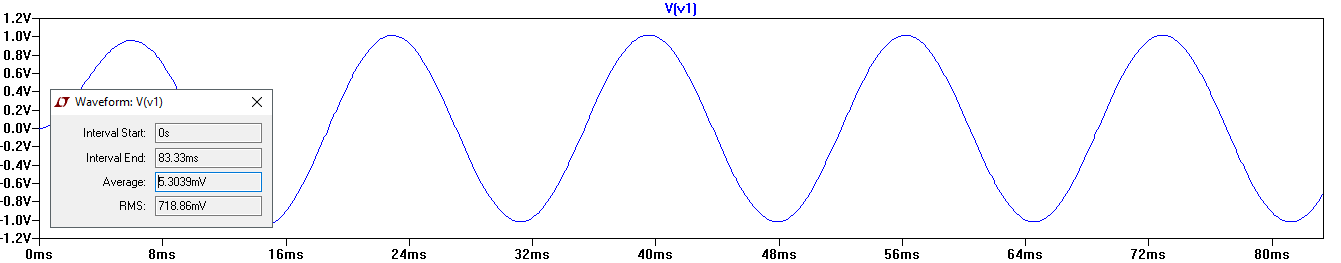
\includegraphics[width=\linewidth]{nod-v1}
\end{figure}
\begin{figure}[H]
    \centering
    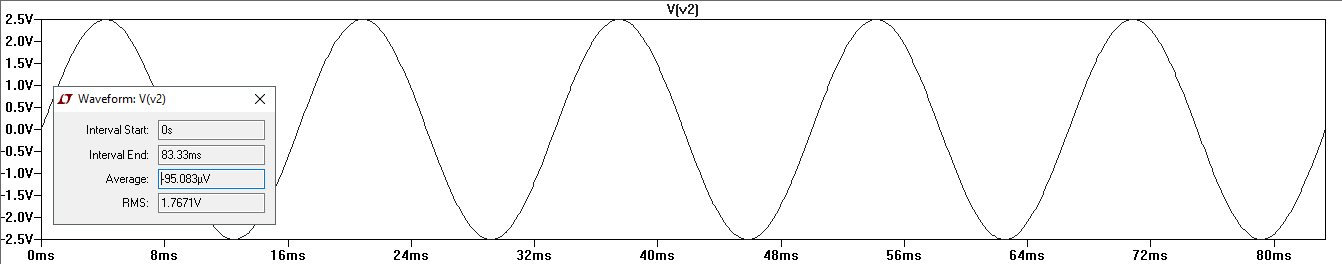
\includegraphics[width=\linewidth]{nod-v2}
\end{figure}
\begin{figure}[H]
    \centering
    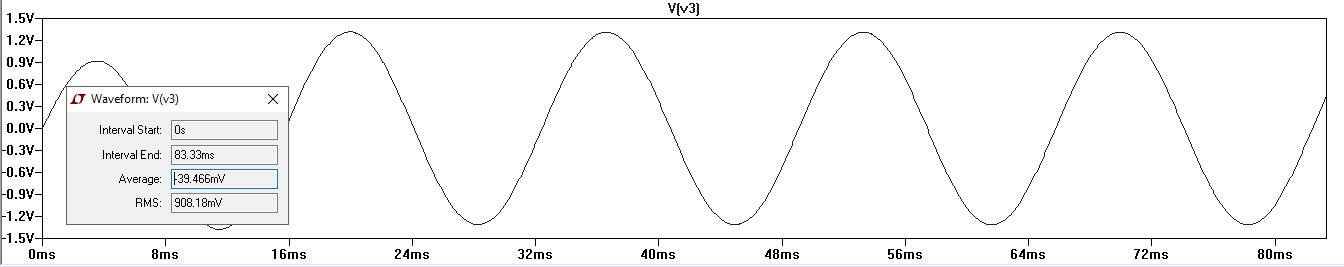
\includegraphics[width=\linewidth]{nod-v3}
\end{figure}
\begin{figure}[H]
    \centering
    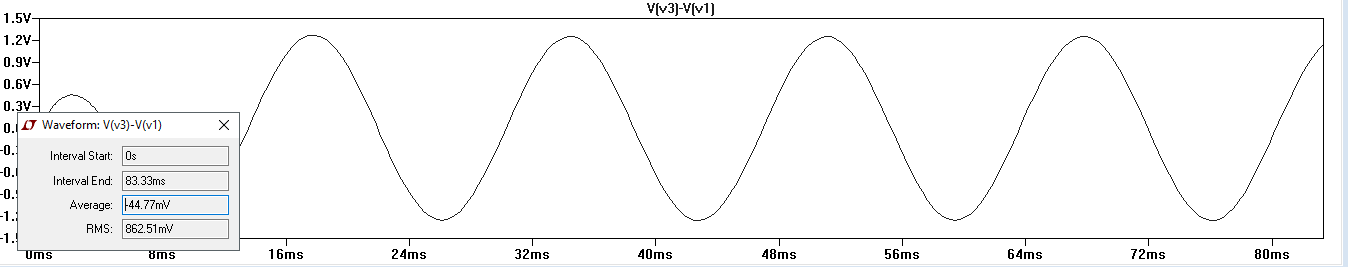
\includegraphics[width=\linewidth]{nod-v13}
\end{figure}
\begin{figure}[H]
    \centering
    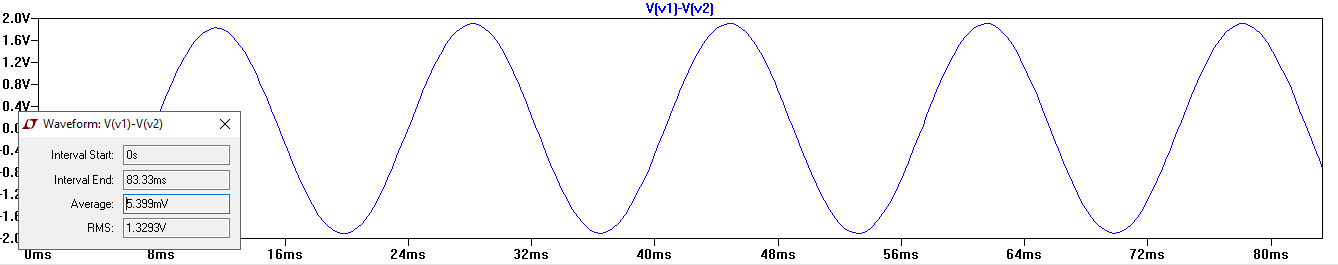
\includegraphics[width=\linewidth]{nod-v21}
\end{figure}
\begin{figure}[H]
    \centering
    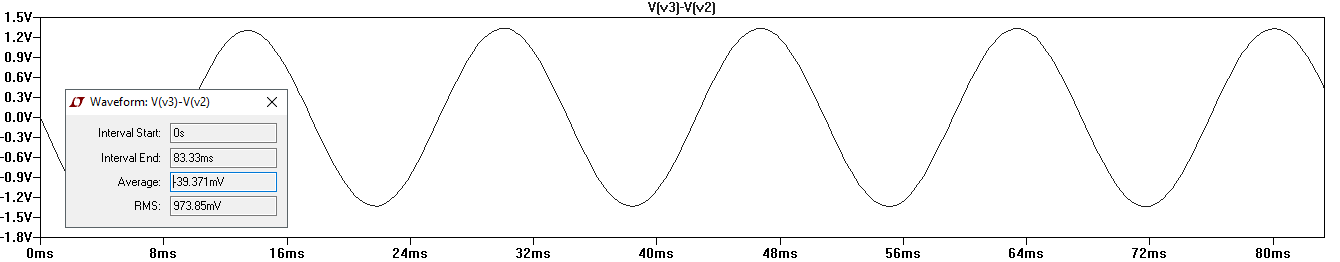
\includegraphics[width=\linewidth]{nod-v23}
\end{figure}
\begin{figure}[H]
    \centering
    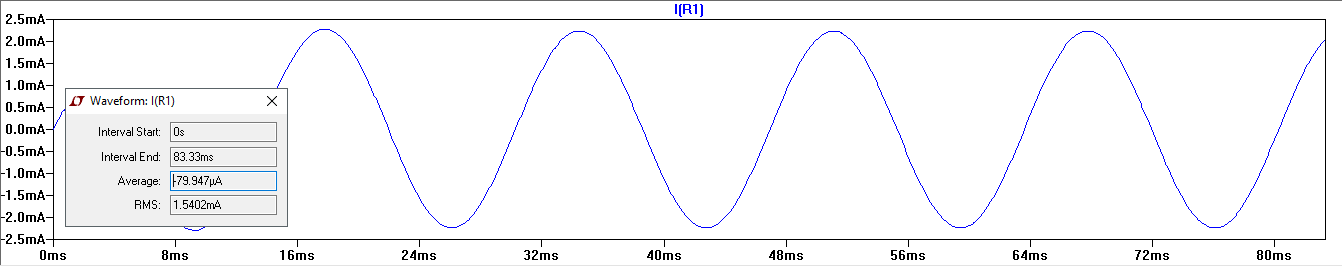
\includegraphics[width=\linewidth]{nod-ir1}
\end{figure}
\begin{figure}[H]
    \centering
    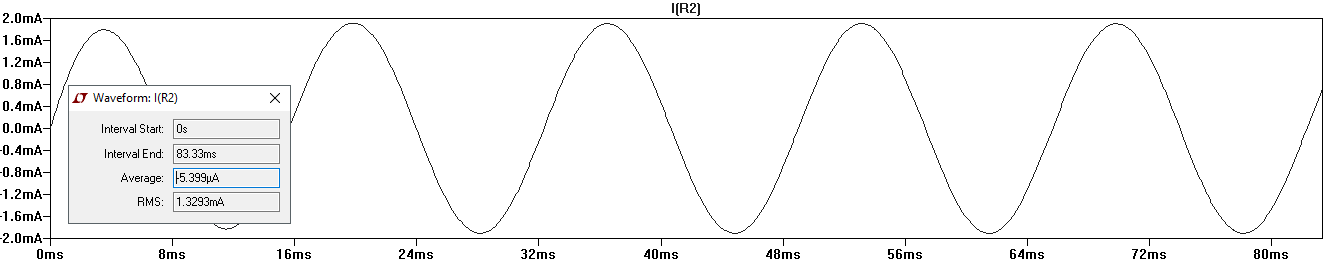
\includegraphics[width=\linewidth]{nod-ir2}
\end{figure}
\begin{figure}[H]
    \centering
    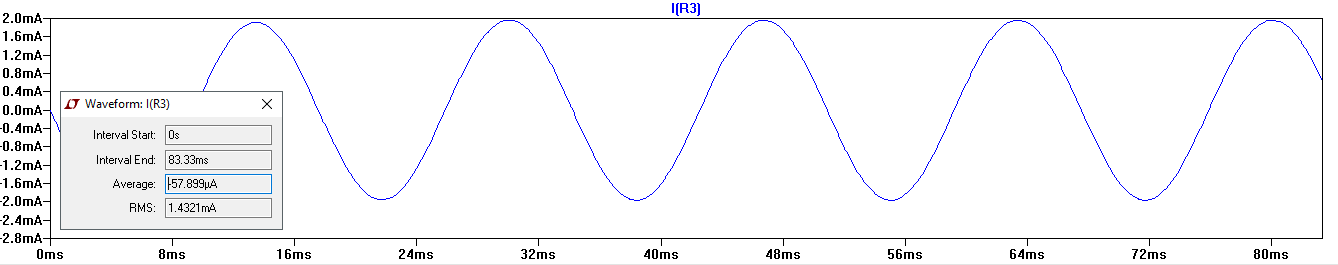
\includegraphics[width=\linewidth]{nod-ir3}
\end{figure}
\begin{figure}[H]
    \centering
    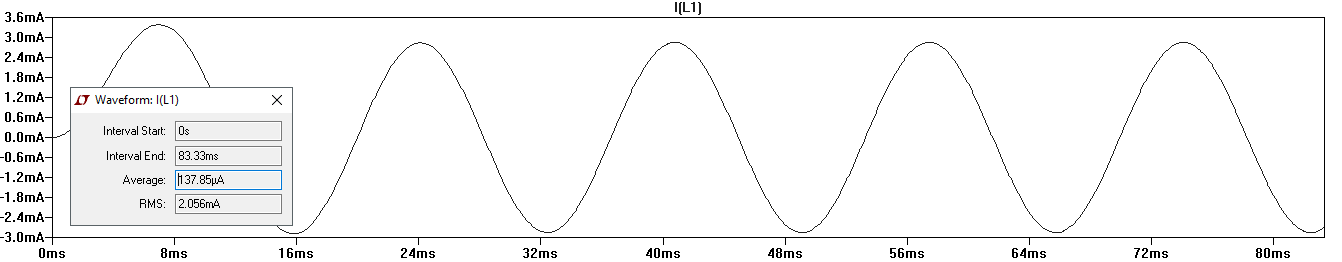
\includegraphics[width=\linewidth]{nod-il}
\end{figure}
\begin{figure}[H]
    \centering
    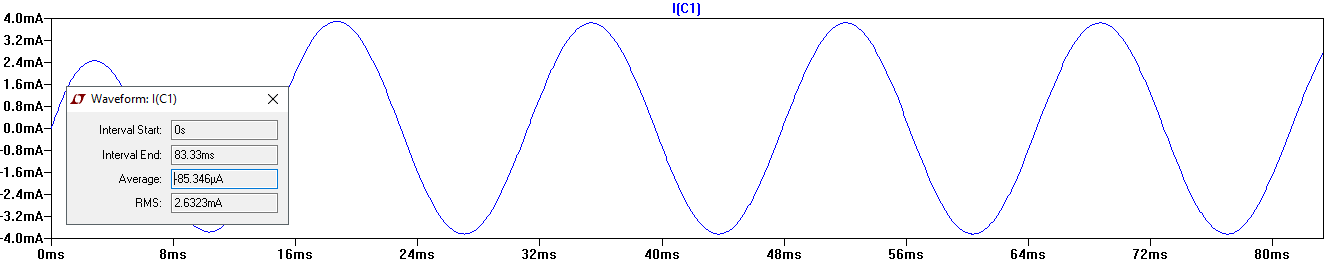
\includegraphics[width=\linewidth]{nod-ic}
\end{figure}
\begin{figure}[H]
    \centering
    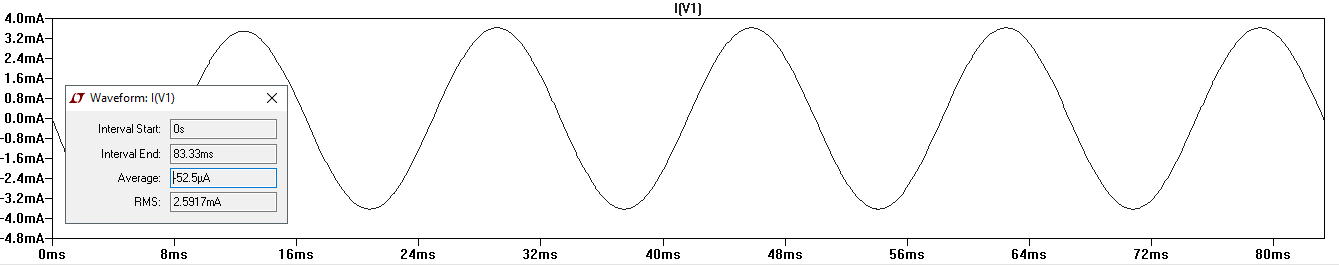
\includegraphics[width=\linewidth]{nod-is}
\end{figure}
\subsubsection{Measurements}
\begin{table}[H]
    \centering
    \begin{tabular}{|c|c|c|c|}
        \hline
        Measurements & Theoretical Value & Measured Value & Simulated Value\\
         & RMS & RMS & RMS\\\hline
        $V_1$ & \SI{0.720}{\volt} & \SI{0.644}{\volt} & \SI{0.718}{\volt}\\\hline 
        $V_2$ & \SI{1.803}{\volt} & \SI{1.659}{\volt} & \SI{1.767}{\volt}\\\hline 
        $V_3$ & \SI{0.928}{\volt} & \SI{0.753}{\volt} & \SI{0.908}{\volt}\\\hline 
        $V_{1,3}$ & \SI{0.886}{\volt} & \SI{0.635}{\volt} & \SI{0.862}{\volt}\\\hline 
        $V_{2,1}$ & \SI{1.347}{\volt} & \SI{1.374}{\volt} & \SI{1.329}{\volt}\\\hline 
        $V_{2,3}$ & \SI{0.945}{\volt} & \SI{0.998}{\volt} & \SI{0.973}{\volt}\\\hline 
        $I_{R1}$ & \SI{1.654}{\milli\ampere} & \SI{1.270}{\milli\ampere} & \SI{1.540}{\milli\ampere}\\\hline 
        $I_{R2}$ & \SI{1.348}{\milli\ampere} & \SI{1.010}{\milli\ampere} & \SI{1.329}{\milli\ampere}\\\hline 
        $I_{R3}$ & \SI{1.389}{\milli\ampere} & \SI{1.350}{\milli\ampere} & \SI{1.432}{\milli\ampere}\\\hline 
        $I_L$ & \SI{2.031}{\milli\ampere} & \SI{2.100}{\milli\ampere} & \SI{2.056}{\milli\ampere}\\\hline 
        $I_C$ & \SI{2.715}{\milli\ampere} & \SI{2.690}{\milli\ampere} & \SI{2.632}{\milli\ampere}\\\hline 
        $I_S$ & \SI{2.570}{\milli\ampere} & \SI{2.530}{\milli\ampere} & \SI{2.592}{\milli\ampere}\\\hline 
    \end{tabular}
    \caption{Measured, simulated and calculated voltage and current values}
\end{table}
\subsection{Mesh analysis}
\subsubsection{Calculations}
Applying KVL in mesh 1:
\begin{gather*}
-V_S+V_L+V_{R4}+V_{R1} = 0\\
-V_S+Z_LI_1+Z_{R4}(I_1+I_2)+Z_{R1}I_1 = 0\\
(Z_L+Z_{R4}+Z_{R1})I_1+I_2-Z_{R4} = V_S
\end{gather*}
substituting values we obtain:
\begin{equation}
    (1560+ 459.929j)I_1-560I_2 = 5
    \label{eq:1}
\end{equation}
Applying KVL in mesh 2:
\begin{gather*}
V_{R2}+V_{R4}+V_C+V_{R3} = 0\\
Z_{R2}I_2+Z_{R4}(I_2-I_1)+Z_CI_2+Z_{R3}I_2 = 0\\
\end{gather*}
substituting values we obtain:
\begin{equation}
    -560I_1+(1360-j265.258)I_2 = 0
    \label{eq:2}
\end{equation}
%%Resolver sistema :c
Finally:
\begin{align*}
    I_1&=\num{1.703e-3}-j\num{5.304e-4}\si{\ampere} =
    \SI{1.784}\measuredangle\ang{-17.29}\si{\milli\ampere}\\
    I_2&=\num{7.168e-4}-j\num{7.862e-5}\si{\ampere} = 
    \SI{0.721}\measuredangle\ang{-6.26}\si{\milli\ampere}\\
\end{align*}
Also, $I_3$ is:
\begin{gather*}
    I_3 = I_1-I_2 = (\num{1.703e-3}+\num{0.717e-3})-j(\num{5.304e-4}+\num{7.862e-5})\\
    \therefore I_3 = \num{9.867e-4}-j\num{6.091e-4}\si{\ampere} =
    \SI{1.159}\measuredangle\ang{-31.69}\si{\milli\ampere}
\end{gather*}
RMS values for each current are the following,for $I_1$:
    \[I_{1(RMS)} = \frac{\SI{1.783}{\milli\ampere}}{\sqrt{2}} = \SI{1.261}{\milli\ampere}\]
for $I_2$:
    \[I_{2(RMS)} = \frac{\SI{0.721}{\milli\ampere}}{\sqrt{2}} = \SI{0.510}{\milli\ampere}\]
for $I_3$:
    \[I_{3(RMS)} = \frac{\SI{1.159}{\milli\ampere}}{\sqrt{2}} = \SI{0.819}{\milli\ampere}\]
Voltage values for all elements are given as follows, for $R_1$:
\begin{gather*}
    V_{R1} = Z_{R1}I_1 = (\SI{1}{\kilo\ohm})(1.784\measuredangle\ang{-17.29}\si{\milli\ampere})\qquad \\
    V_{R1} = 1.784\measuredangle\ang{-17.29}\si{\volt}\\
    \therefore V_{R1(RMS)} = \frac{\SI{1.784}{\volt}}{\sqrt{2}} = \SI{1.261}{\volt}
\end{gather*}
for $R_2$:
\begin{gather*}
    V_{R2} = Z_{R2}I_2 = (\SI{470}{\ohm})(0.721\measuredangle\ang{-6.26}\si{\milli\ampere})\qquad \\
    V_{R2} = 0.339\measuredangle\ang{-6.26}\si{\volt}\\
    \therefore V_{R2(RMS)} = \frac{\SI{0.339}{\volt}}{\sqrt{2}} = \SI{0.240}{\volt}
\end{gather*}
for $R_3$:
\begin{gather*}
    V_{R3} = Z_{R3}I_2 = (\SI{330}{\ohm})(0.721\measuredangle\ang{-6.26}\si{\milli\ampere})\qquad \\
    V_{R3} = 0.238\measuredangle\ang{-6.26}\si{\volt}\\
    \therefore V_{R3(RMS)} = \frac{\SI{0.238}{\volt}}{\sqrt{2}} = \SI{0.168}{\volt}
\end{gather*}
for $R_4$:
\begin{gather*}
    V_{R4} = Z_{R4}I_3 = (\SI{560}{\ohm})(1.159\measuredangle\ang{-31.69}\si{\milli\ampere})\qquad \\
    V_{R4} = 0.649\measuredangle\ang{-31.69}\si{\volt}\\
    \therefore V_{R4(RMS)} = \frac{\SI{0.649}{\volt}}{\sqrt{2}} = \SI{0.459}{\volt}
\end{gather*}
for $L$:
\begin{gather*}
    V_{L} = Z_{L}I_1 = (459.929\measuredangle\ang{90}\si{\ohm})(1.784\measuredangle\ang{-17.29}\si{\milli\ampere})\qquad \\
    V_{L} = 0.820\measuredangle\ang{72.71}\si{\volt}\\
    \therefore V_{L(RMS)} = \frac{\SI{0.820}{\volt}}{\sqrt{2}} = \SI{0.580}{\volt}
\end{gather*}
for $C$:
\begin{gather*}
    V_{C} = Z_{C}I_2 = (265.268\measuredangle\ang{-90}\si{\ohm})(0.721\measuredangle\ang{-6.26}\si{\milli\ampere})\qquad \\
    V_{C} = 0.191\measuredangle\ang{-96.26}\si{\volt}\\
    \therefore V_{C(RMS)} = \frac{\SI{0.191}{\volt}}{\sqrt{2}} = \SI{0.135}{\volt}
\end{gather*}
for $V_S$:
\begin{gather*}
    V_{S} = 2.5\measuredangle\ang{0}\si{\volt}\\
    \therefore V_{S(RMS)} = \frac{\SI{2.5}{\volt}}{\sqrt{2}} = \SI{1.768}{\volt}
\end{gather*}
\subsubsection{Simulations}
\begin{figure}[H]
    \centering
    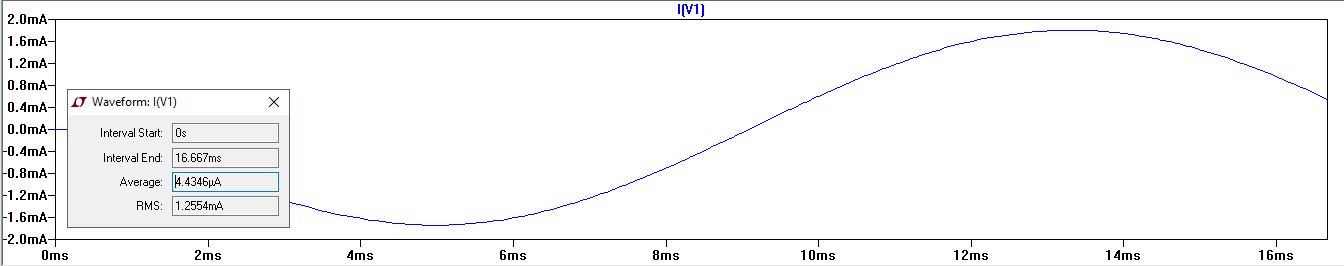
\includegraphics[width=\linewidth]{mesh-i1}
\end{figure}
\begin{figure}[H]
    \centering
    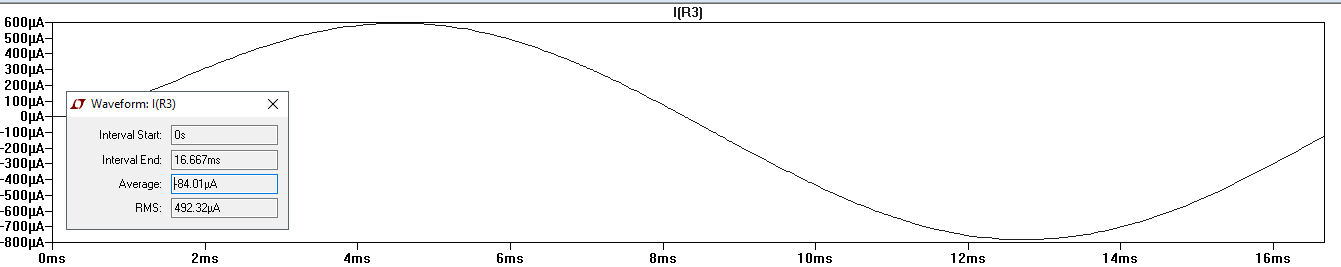
\includegraphics[width=\linewidth]{mesh-i2}
\end{figure}
\begin{figure}[H]
    \centering
    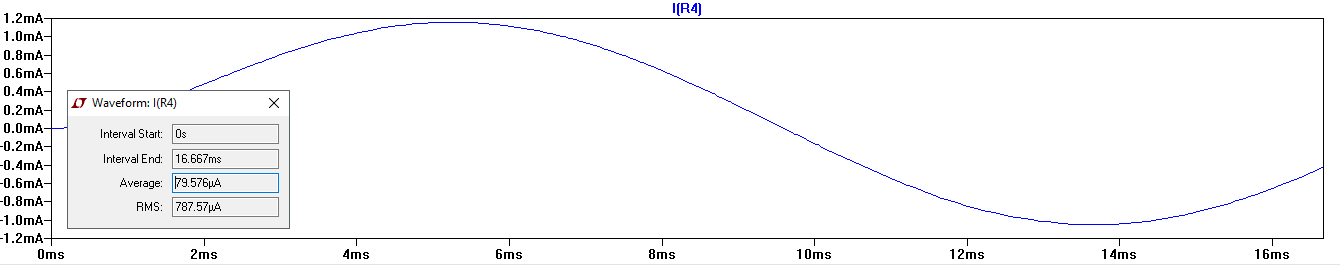
\includegraphics[width=\linewidth]{mesh-i3}
\end{figure}
\begin{figure}[H]
    \centering
    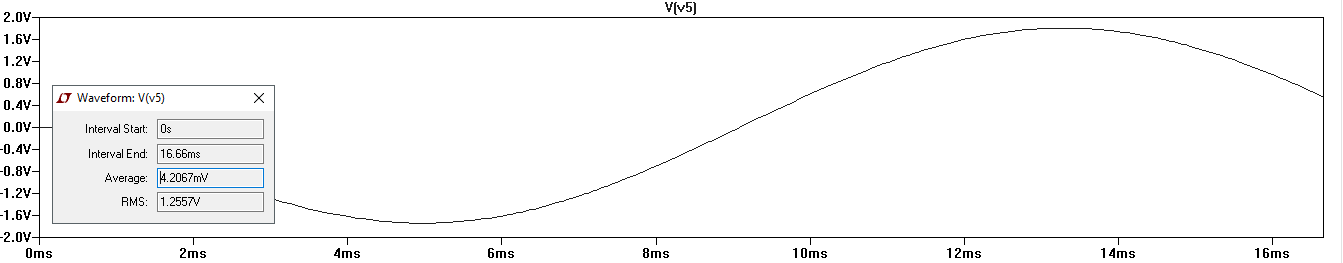
\includegraphics[width=\linewidth]{mesh-vr1}
\end{figure}
\begin{figure}[H]
    \centering
    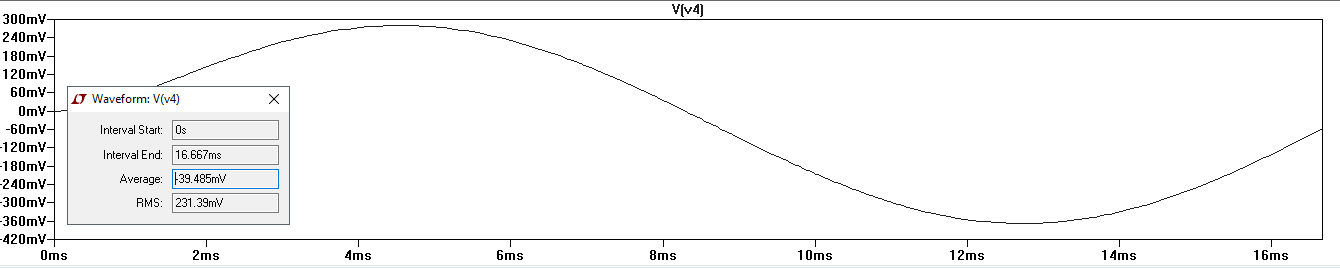
\includegraphics[width=\linewidth]{mesh-vr2}
\end{figure}
\begin{figure}[H]
    \centering
    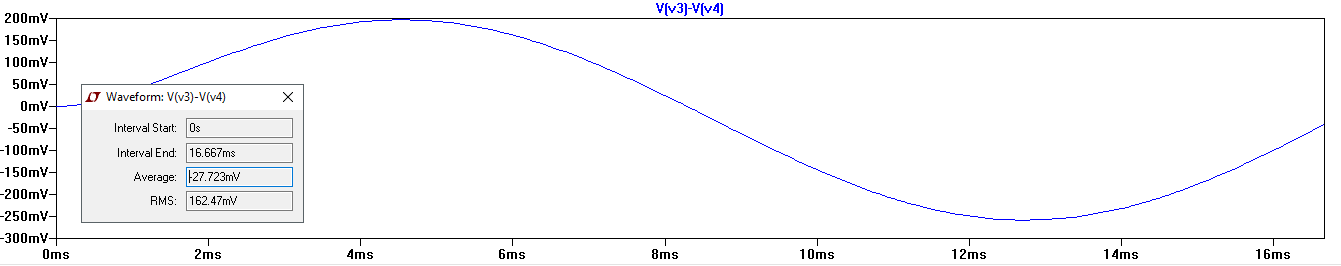
\includegraphics[width=\linewidth]{mesh-vr3}
\end{figure}
\begin{figure}[H]
    \centering
    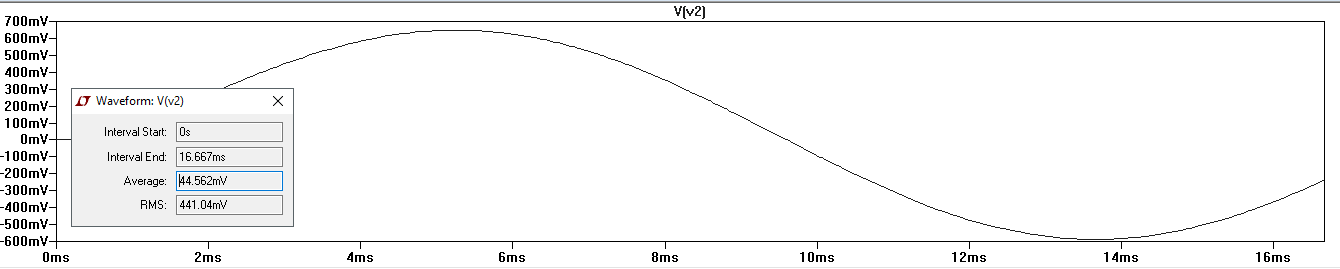
\includegraphics[width=\linewidth]{mesh-vr4}
\end{figure}
\begin{figure}[H]
    \centering
    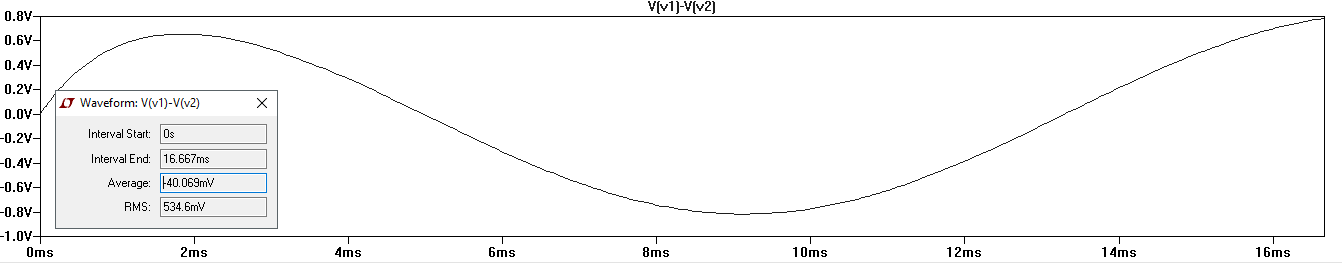
\includegraphics[width=\linewidth]{mesh-vl}
\end{figure}
\begin{figure}[H]
    \centering
    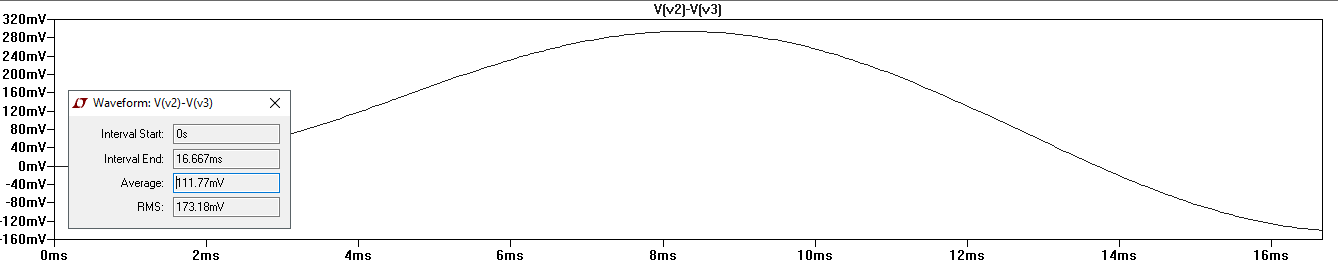
\includegraphics[width=\linewidth]{mesh-vc}
\end{figure}
\begin{figure}[H]
    \centering
    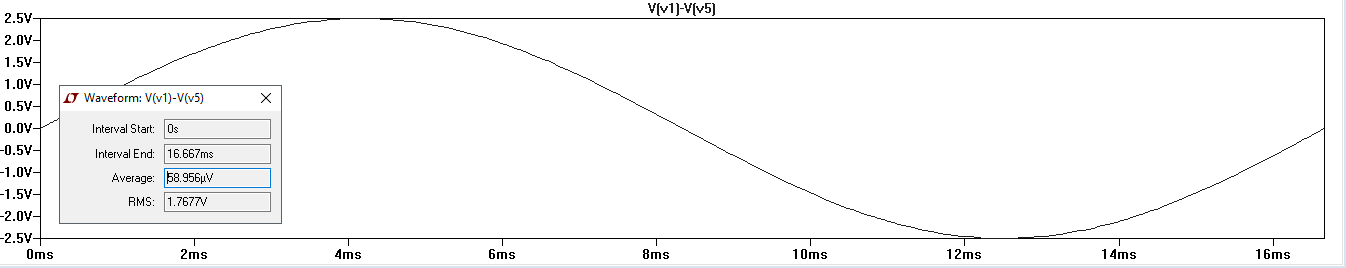
\includegraphics[width=\linewidth]{mesh-vs}
\end{figure}
\subsubsection{Measurements}
\begin{table}[H]
    \centering
    \begin{tabular}{|c|c|c|c|}
        \hline
        Measurements & Theoretical Value & Measured Value & Simulated Value\\
         & RMS & RMS & RMS\\\hline
        $I_1$ & \SI{1.261}{\milli\ampere} & \SI{1.180}{\milli\ampere} & \SI{1.255}{\milli\ampere}\\\hline 
        $I_2$ & \SI{0.510}{\milli\ampere} & \SI{0.420}{\milli\ampere} & \SI{0.492}{\milli\ampere}\\\hline 
        $I_3$ & \SI{0.819}{\milli\ampere} & \SI{0.750}{\milli\ampere} & \SI{0.787}{\milli\ampere}\\\hline 
        $V_{R1}$ & \SI{1.261}{\volt} & \SI{1.210}{\volt} & \SI{1.255}{\volt}\\\hline 
        $V_{R2}$ & \SI{0.240}{\volt} & \SI{0.213}{\volt} & \SI{0.231}{\volt}\\\hline 
        $V_{R3}$ & \SI{0.168}{\volt} & \SI{0.122}{\volt} & \SI{0.162}{\volt}\\\hline 
        $V_{R4}$ & \SI{0.459}{\volt} & \SI{0.452}{\volt} & \SI{0.441}{\volt}\\\hline 
        $V_L$ & \SI{0.580}{\volt} & \SI{0.455}{\volt} & \SI{0.534}{\volt}\\\hline 
        $V_C$ & \SI{0.135}{\volt} & \SI{0.101}{\volt} & \SI{0.173}{\volt}\\\hline 
        $V_S$ & \SI{1.768}{\volt} & \SI{1.752}{\volt} & \SI{1.768}{\volt}\\\hline 
    \end{tabular}
    \caption{Measured, simulated and calculated voltage and current values}
\end{table}
\subsection{Voltage divider}
\subsubsection{Calculations}
Now that we have all the impedances we can calculate the voltage in each component
using the voltage divider equation. For $R_1$ we have:
\begin{gather*}
    V_{C} = \frac{V_S}{Z_R+Z_C+Z_L}\cdot Z_C = \frac{2.5}{1000+j194.66}\cdot -j265.268\si{\ohm} =
    \frac{2.5}{1018.770\measuredangle\ang{11.01}}\cdot 265.268\measuredangle\ang{-90}\si{\ohm}\\
    V_{C} = 0.651\measuredangle\ang{-101.01}\\
    \therefore V_{C(RMS)} = \frac{\SI{0.651}{\volt}}{\sqrt{2}} = \SI{0.460}{\volt}
\end{gather*}
\begin{gather*}
    V_{R} = \frac{V_S}{Z_R+Z_C+Z_L}\cdot Z_R = \frac{2.5}{1000+j194.66}\cdot 10000\si{\ohm} =
    \frac{2.5}{1018.770\measuredangle\ang{11.01}}\cdot 1000\si{\ohm}\\
    V_{R} = 2.454\measuredangle\ang{-11.01}\\
    \therefore V_{R(RMS)} = \frac{\SI{2.454}{\volt}}{\sqrt{2}} = \SI{1.735}{\volt}
\end{gather*}
\begin{gather*}
    V_{L} = \frac{V_S}{Z_R+Z_C+Z_L}\cdot Z_L = \frac{2.5}{1000+j194.66}\cdot j459.929\si{\ohm} =
    \frac{2.5}{1018.770\measuredangle\ang{11.01}}\cdot 459.929\measuredangle\ang{90}\\
    V_{L} = 1.129\measuredangle\ang{78.99}\\
    \therefore V_{L(RMS)} = \frac{\SI{1.129}{\volt}}{\sqrt{2}} = \SI{0.798}{\volt}
\end{gather*}
Then, in each node the voltage is given as follows, for $V_1$ is the same value as the votage
source, therefore:
\begin{gather*}
    V_1 = \SI{2.5}{\volt}\measuredangle\ang{0}\\
    \therefore V_{1(RMS)} = \frac{\SI{2.5}{\volt}}{\sqrt{2}} = \SI{1.768}{\volt}
\end{gather*}
for $V_2$:
\begin{gather*}
    V_2 = V_1 - V_L = \SI{2.5}{\volt}-(-0.124-j0.639\si{\volt}) = 2.624+j0.639\si{\volt} =
    2.701\measuredangle\ang{13.68}\\
    \therefore V_{2(RMS)} = \frac{\SI{2.701}{\volt}}{\sqrt{2}} = \SI{1.910}{\volt}
\end{gather*}
for $V_3$:
\begin{gather*}
    V_3 = V_2 - V_R = 2.624+j0.639\si{\volt}-2.409-j0.469\si{\volt}) = 0.216+j1.108\si{\volt} =
    1.129\measuredangle\ang{78.985}\\
    \therefore V_{3(RMS)} = \frac{\SI{1.129}{\volt}}{\sqrt{2}} = \SI{0.798}{\volt}
\end{gather*}
Finally, current is given by:
\begin{gather*}
    I_T = \frac{V_S}{Z_R} = \frac{\SI{2.5}{\volt}}{1000} = \SI{2.5}{\milli\ampere}
    \therefore I_T = \frac{\SI{2.5}{\milli\ampere}}{\sqrt{2}} = \SI{1.767}{\milli\ampere}
\end{gather*}
\subsubsection{Simulations}
\begin{figure}[H]
    \centering
    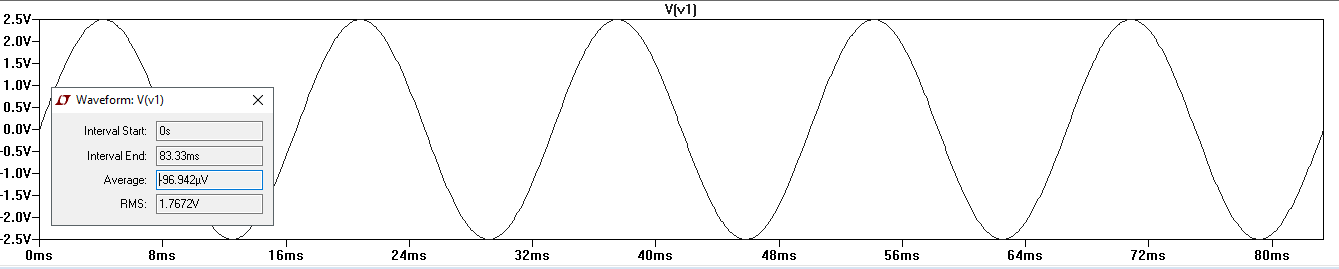
\includegraphics[width=\linewidth]{div-v1}
\end{figure}
\begin{figure}[H]
    \centering
    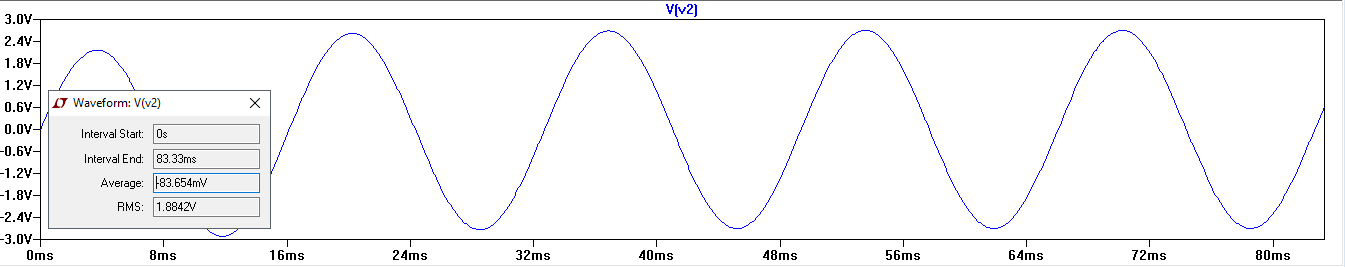
\includegraphics[width=\linewidth]{div-v2}
\end{figure}
\begin{figure}[H]
    \centering
    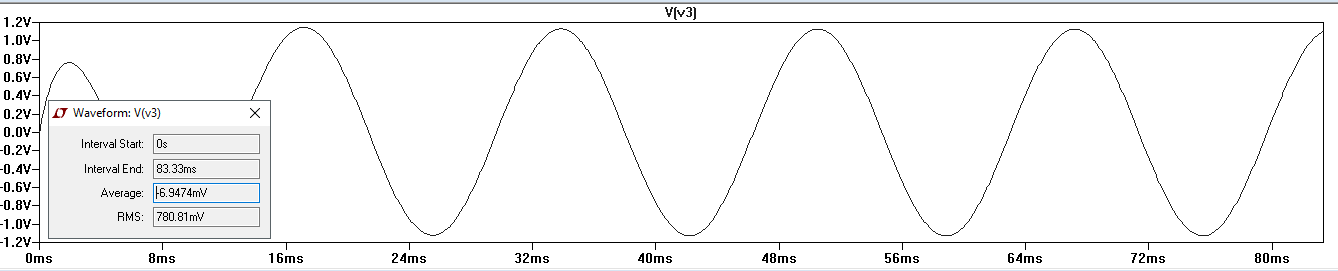
\includegraphics[width=\linewidth]{div-v3}
\end{figure}
\begin{figure}[H]
    \centering
    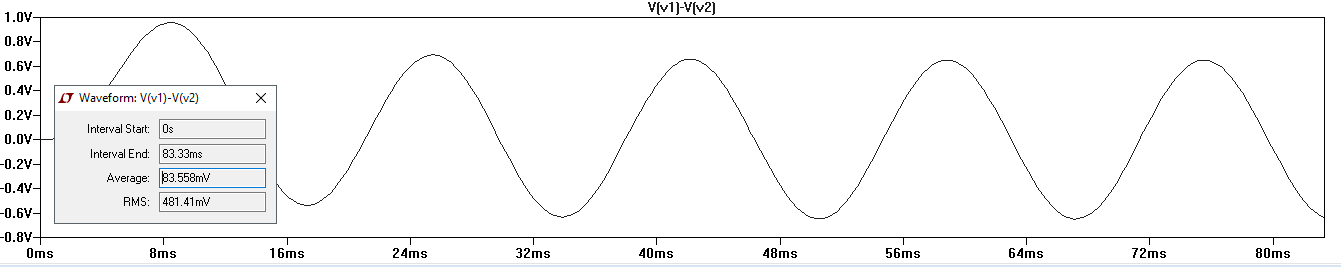
\includegraphics[width=\linewidth]{div-cap}
\end{figure}
\begin{figure}[H]
    \centering
    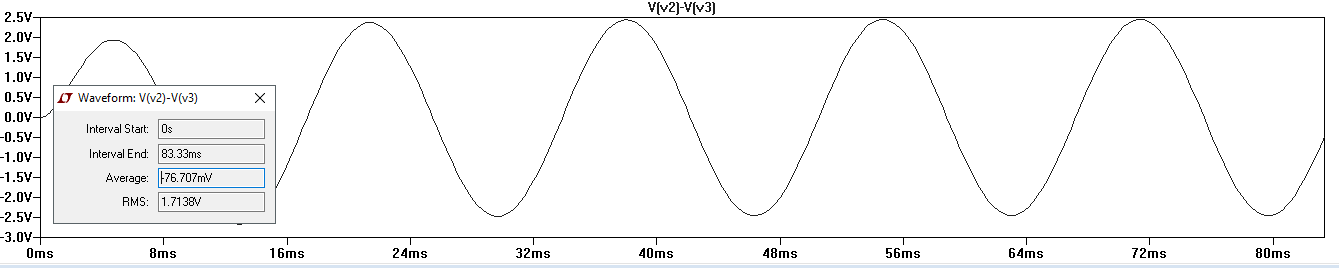
\includegraphics[width=\linewidth]{div-res}
\end{figure}
\begin{figure}[H]
    \centering
    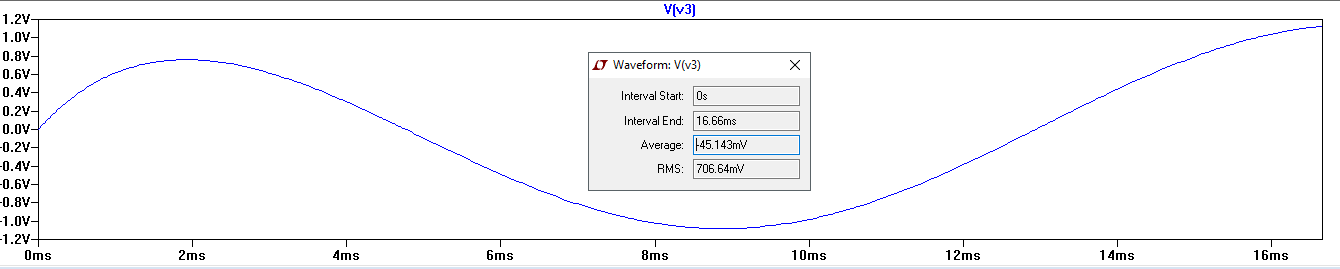
\includegraphics[width=\linewidth]{div-ind}
\end{figure}
\begin{figure}[H]
    \centering
    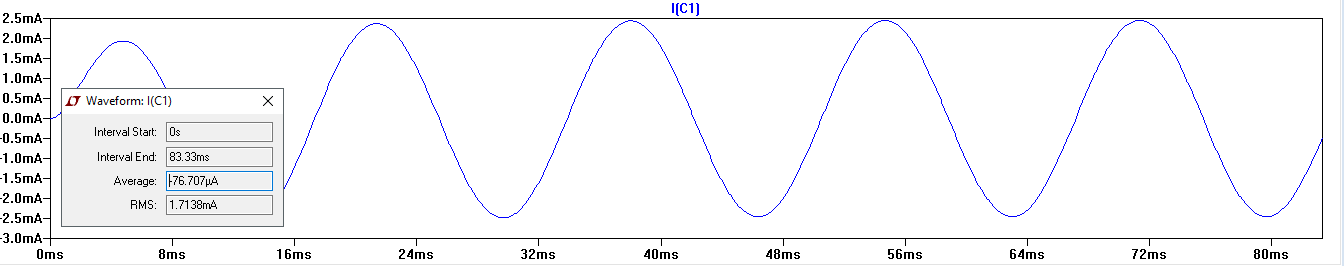
\includegraphics[width=\linewidth]{div-curr}
\end{figure}
\subsubsection{Measurements}
\begin{table}[H]
    \centering
    \begin{tabular}{|c|c|c|c|c|}
        \hline
        Measurements & Theoretical Value & Measured Value & Simulated Value & Error($\Delta V$) \\
         & RMS & RMS & RMS & \\\hline
        $V_1$ & \SI{1.768}{\volt} & \SI{1.735}{\volt} & \SI{1.767}{\volt} & \SI{0.033}{\volt}\\\hline 
        $V_2$ & \SI{1.910}{\volt} & \SI{1.767}{\volt} & \SI{1.884}{\volt} & \SI{0.143}{\volt}\\\hline 
        $V_3$ & \SI{0.798}{\volt} & \SI{0.638}{\volt} & \SI{0.780}{\volt} & \SI{0.160}{\volt}\\\hline 
        $V_C$ & \SI{0.460}{\volt} & \SI{0.328}{\volt} & \SI{0.481}{\volt} & \SI{0.132}{\volt}\\\hline 
        $V_R$ & \SI{1.735}{\volt} & \SI{1.209}{\volt} & \SI{1.714}{\volt} & \SI{0.526}{\volt}\\\hline 
        $V_L$ & \SI{0.798}{\volt} & \SI{0.638}{\volt} & \SI{0.707}{\volt} & \SI{0.160}{\volt}\\\hline 
        $I_T$ & \SI{1.767}{\milli\ampere} & \SI{1.580}{\milli\ampere} & \SI{1.714}{\milli\ampere} &
        \SI{0.187}{\milli\ampere}\\\hline 
    \end{tabular}
    \caption{Measured, simulated and calculated voltage and current values}
\end{table}
\end{document}
